

\Large{The Experiment}
%TODO Get rid of 4panel, put the top left picture, include text/caption explaining the setting based on picture added
\normalsize
\begin{figure}
\setlength{\belowcaptionskip}{-7pt}
\begin {center}
\begin {tikzpicture}[-latex ,auto ,node distance =3cm and 4cm ,on grid ,
semithick ,
state/.style ={ circle ,fill=black!20, minimum width =3 cm}]
\node[state] (C){$Sold$};
\node[state] (A) [above left=of C,align=center] {Recession};
\node[state] (B) [above right =of C,align=center] {Booming};
\coordinate[below of=A] (AA);
\coordinate[below of=B] (BB);
\coordinate[below of=AA] (D);
\coordinate[below of=BB] (E);


\path (A) edge [loop left, line width=2mm, align=center] node[left] {wait \\ $0.86$} (A);
\path (A) edge [bend left = -25,line width=2mm,align=center] node[below =0.25 cm] {sell\\$1.0$} (C);
\path (A) edge [bend left =25,line width=2mm,align=center] node[above] {wait\\$0.14$} (B);

\path (B) edge [loop right,line width=2mm,align=center] node[right] {wait\\$1.0$} (B);
\path (B) edge [bend right = -25,line width=2mm,align=center] node[below =0.25 cm] {sell\\$1.0$} (C);

%\fill[gray!40!white, opacity=0.5] (-6,-1) rectangle (5,6);

\path (A) edge [bend right =25,line width=2mm, dashed] node[left] {$Observation$} (D);
\path (B) edge [bend left  =25,line width=2mm, dashed] node[right] {$Observation$} (E);
\end{tikzpicture}
\end{center}
 \caption{The experiment setup. The market has three states, \textit{recession} and \textit{booming} and \textit{sold}. The market starts in recession and iteratively transitions are performed. At each transition subjects are shown an observation from the current state and can choose between \textit{wait} and \textit{sell}. The experiments ends when subjects sell and they receive a reward based on the last market state.}
\end{figure}
\begin{itemize}
    \item In a simulated housing market, subjects needed to decide when to sell a house.
    \item Waiting decreases risk, but increases costs.
    \item 24 participants performed two different scenarios.
\end{itemize}


\begin{figure}
\setlength{\belowcaptionskip}{-7pt}
\centering
\begin{subfigure}{.5\textwidth}
  \centering
  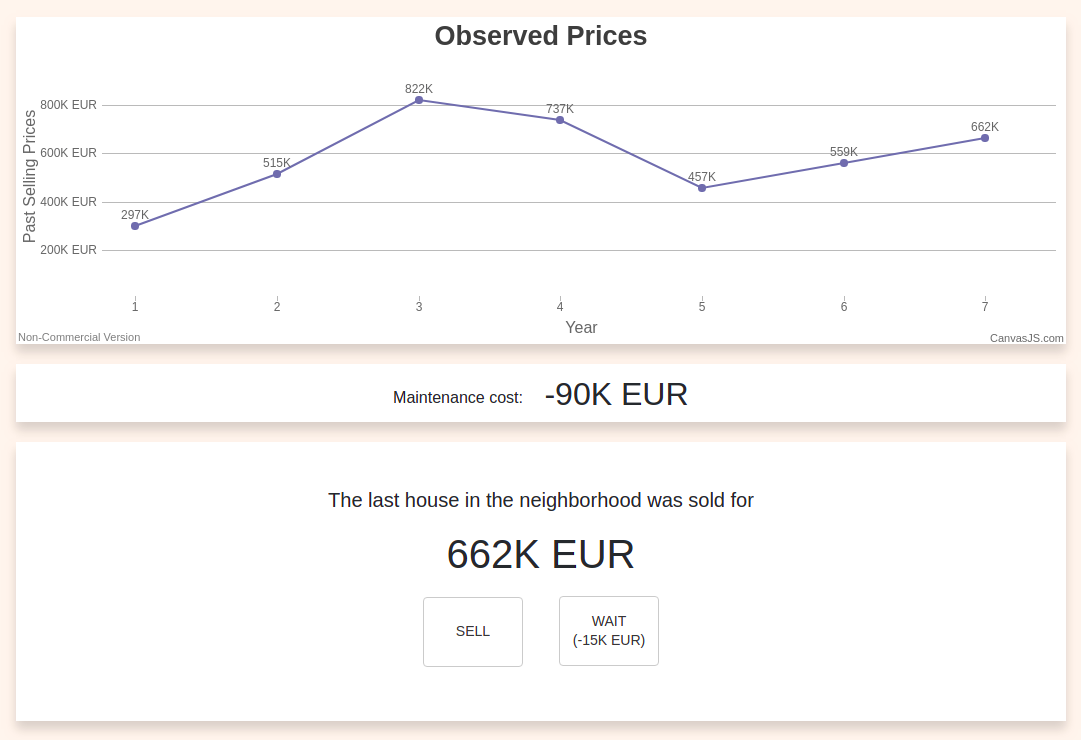
\includegraphics[width=0.95\textwidth]{img/methods/experiment_obs_1.png}
  \caption{Observation experiment}
\end{subfigure}%
\begin{subfigure}{.5\textwidth}
  \centering
 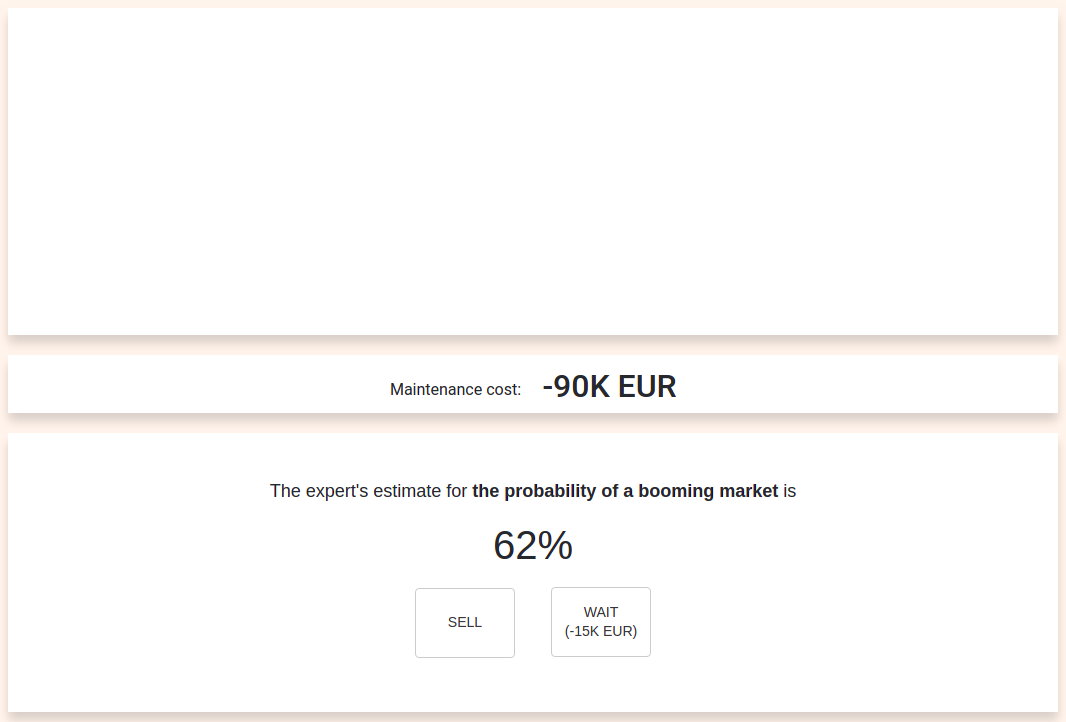
\includegraphics[width=0.95\textwidth]{img/methods/experiment_bel_1.png}
  \caption{Bayesian estimate experiment}
\end{subfigure}
\caption{The two experiment scenarios and their respective UI. In (a) subjects are shown the observation history at the top and a new observation at the bottom. In (b) they see the Bayesian estimate based on the observation history.}
\end{figure}
\Large{The Agent}
\normalsize
\begin{itemize}
    \item Simplify POMDP into a MDP by Bayesian estimates.
    \begin{figure}
    \setlength{\belowcaptionskip}{-3pt}
        \centering
        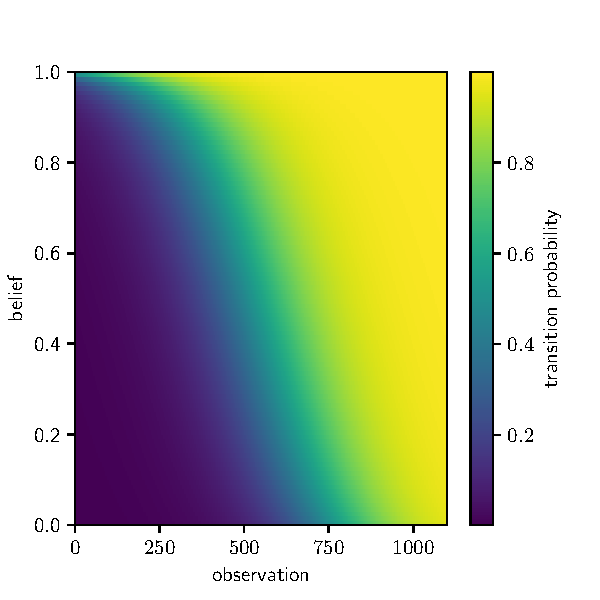
\includegraphics[scale=0.9]{img/belief_table.pdf}
        \caption{The updated believe $b'$ given a current believe $b$ and an observation $o$, calculated using Bayesian estimation}
    \end{figure}
    \item Solve the MDP with value iteration on an augmented state space. \cite{bauerle}
    \begin{flalign}
    V^{n}_{U}(b,w) &= U(w)\tag{Initalization} \\
    V^{n-1}_{U}(b,w) &= \max_{a \in A}(\sum_{o \in O}{P(o|b)V^{n}_{U}(b', w + r(a))}) \tag{Iteration}
    \end{flalign}
    
    \item Different utility functions model different behaviors
    \begin{itemize}
    	\item Time independent (risk parameter $\lambda$)
	 \begin{flalign}
    		U(w)  = \left(1-exp(- \lambda w)\right) / \lambda &&\tag{Exponential utility}
	 \end{flalign}
	 \item Time dependent (risk parameter $\lambda (w)$), \cite{Penner2008Dynamic}
	 \begin{flalign}
    		U(w) &= \left(1-exp(- \lambda(w) w)\right) / \lambda(w)  && \tag{Dynamic Exponential utility}
	 \end{flalign}
	 \item Belief independent (scaling $a$, shift $b$)
	 \begin{flalign}
    		U(w) &= \sinh(a (w-b)) && \tag{Hyperbolic utility}
	 \end{flalign}
    \end{itemize}
\end{itemize}
